\problem{48}{(สอวน ม.4 รอบที่ 1 2555) $A$ กับ $B$ อยู่ห่างกัน $l$ ทั้งคู่เริ่มออกวิ่งไปทางขวาด้วยความเร่งคงที่ $a$ และ $b$ ตามลำดับ $A$ จะต้องกวด $B$ อยู่นานเท่าใดจึงทัน $B$ กำหนดว่า $a>b$}
\begin{center}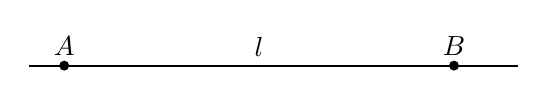
\begin{tikzpicture}[scale=.9]\draw[thick](-.5,0)--(6.4,0);\fill(0,0)circle(2pt)node[above]{$A$};\fill(5.5,0)circle(2pt)node[above]{$B$};\node at (2.75,.27){$l$};\end{tikzpicture}\end{center}
